\section{Introduction}

\subsection{A Database in MySQL}

MDPX Database is a data management web application developed by the Plasma Science Laboratory of Physics Department, in conjunction with the Computer Science Department, at Auburn University for storing data for magnetized dusty plasma experiments. The database tracks 3 kinds of data:

\begin{enumerate}
\item Experiment Configuration: parts and instruments used in an experiments along with set points.
\item Research Data: measurements and feedbacks from instruments.
\item User Management: user information and access permissions for the web front-end.
\end{enumerate}

The database is initially designed using the relational data model and currently running on MySQL database server. We chose relational data model and MySQL database server because of the maturity of the technology. As a software developer who has been writing software and making web applications for the past 10 years, I have witnessed the growth in adoption of MySQL for new software projects since its early inception in the 1990s. MySQL also has the reputation of being able to evaluate queries very fast. In addition, there are software projects that only support MySQL as the database back-end.

Despite the advantages, we are running into limitations of relational database. One of the major limitation is the complexity of schema due to the rigidity of the database structure. This problem stemmed from the fact that our database keeps track of different kind of plasma experiment instruments (also called parts, for short) as well as properties of these parts. Each kind of parts has unique properties, which are not easily captured in the rigid structure of relational database.

The approach we took to accommodate this is shown in Figure~\ref{setup-parts-a}. In this approach, we store attributes of different parts in one table. As shown in the figure, we store camera setup information in one table, and probe setup information in another, and there is a master table that keep track of all setup parts. This approach is simple to work with and works for small number of part types, but becomes increasingly complicated as the number of parts gets large.

\begin{figure}[h]
    \centering
    \subfigure[One table for each part type]
    {
        \label{setup-parts-a}
        %\begin{minipage}[h!]{0.5\textwidth}
        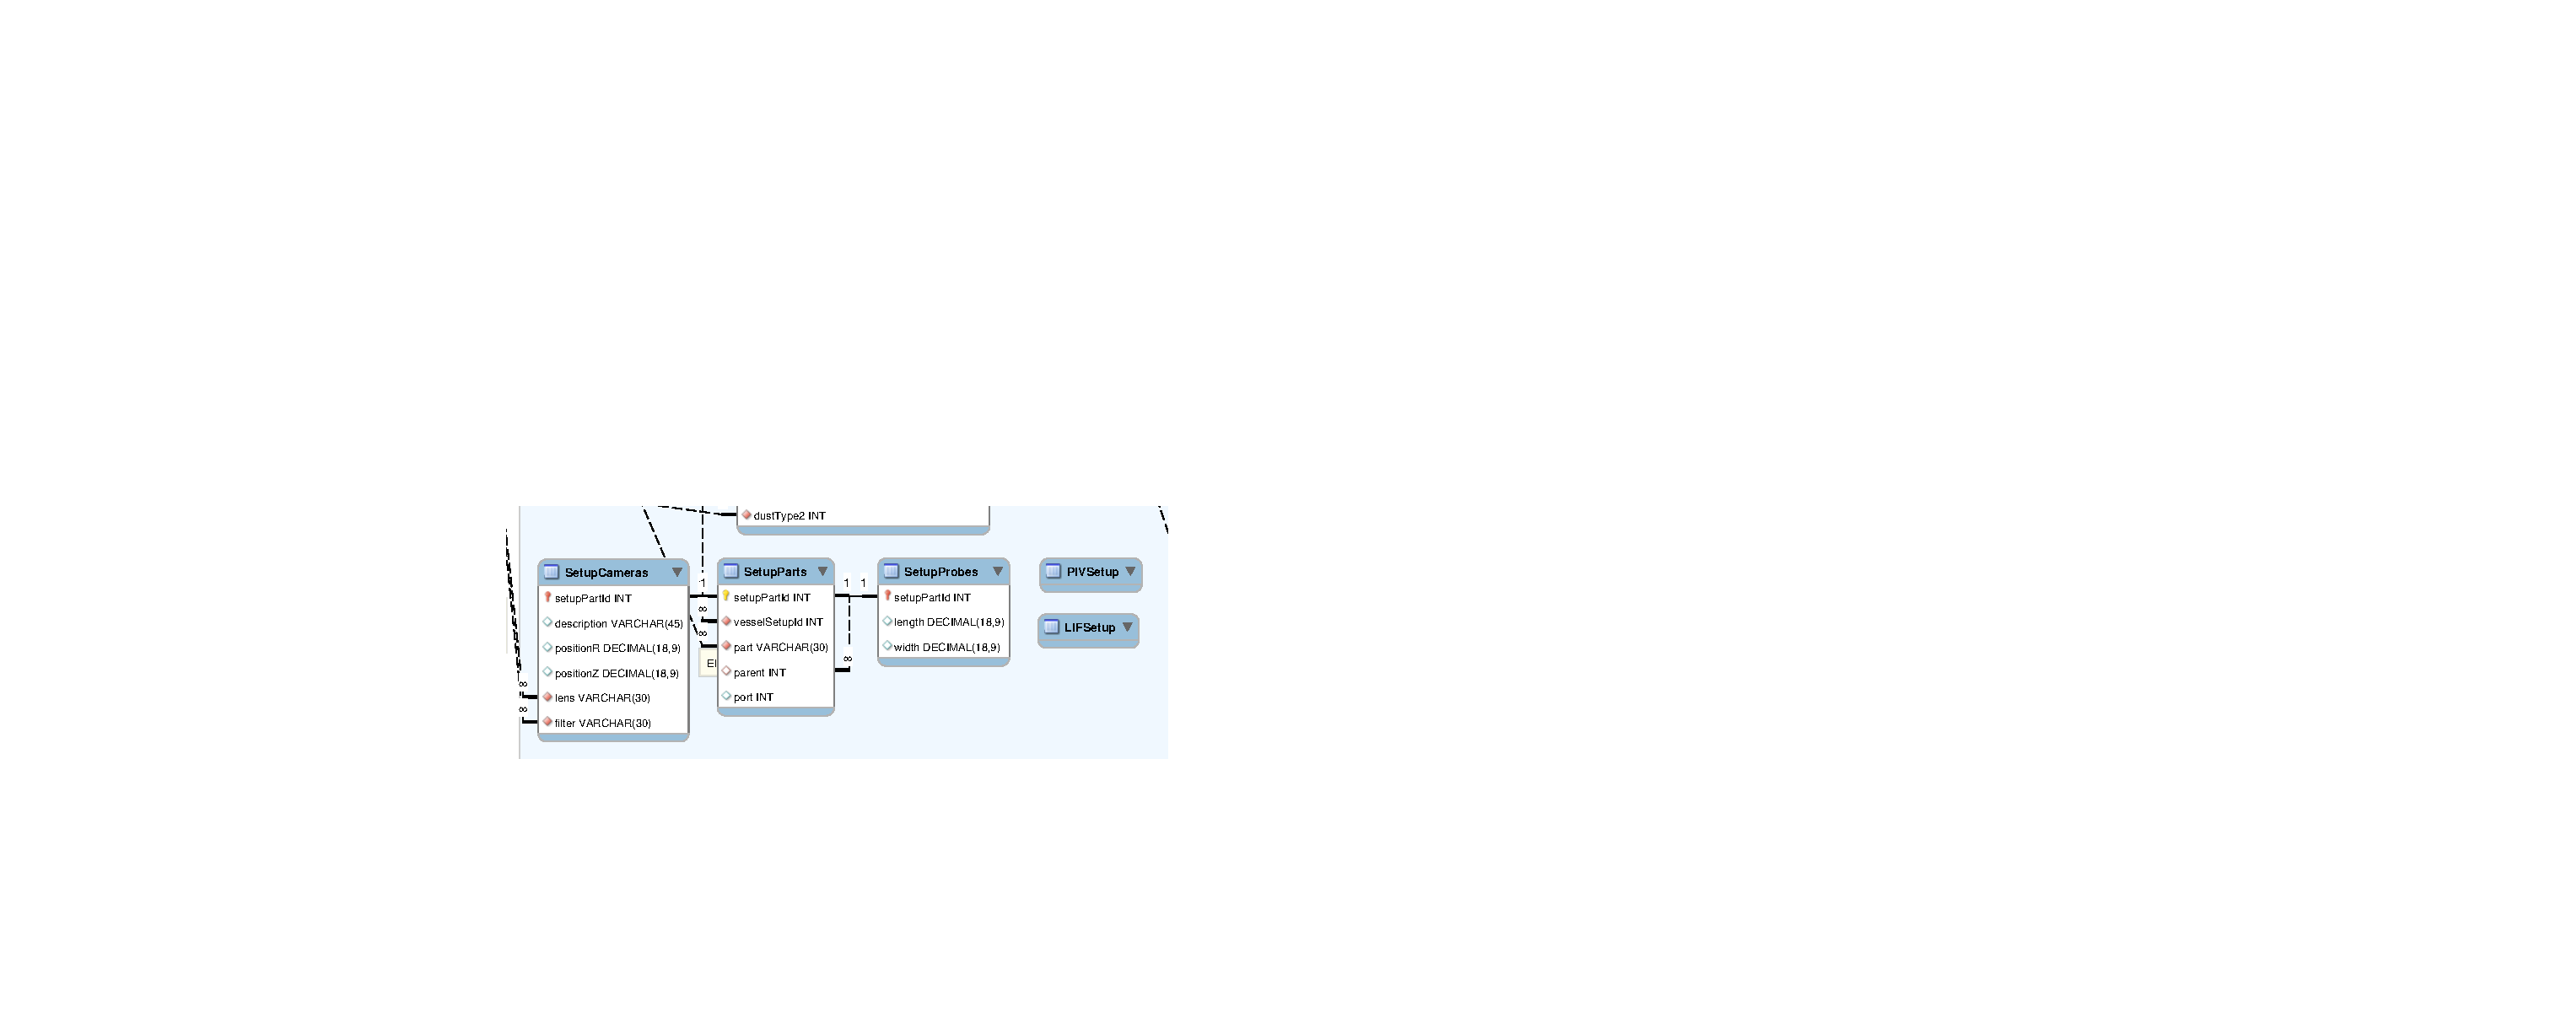
\includegraphics[width=3in]{figures/setup-parts.pdf}
        %\end{minipage}
    }
    \subfigure[Property table for all parts]
    {
        \label{setup-parts-b}
        %\begin{minipage}[h!]{0.5\textwidth}
        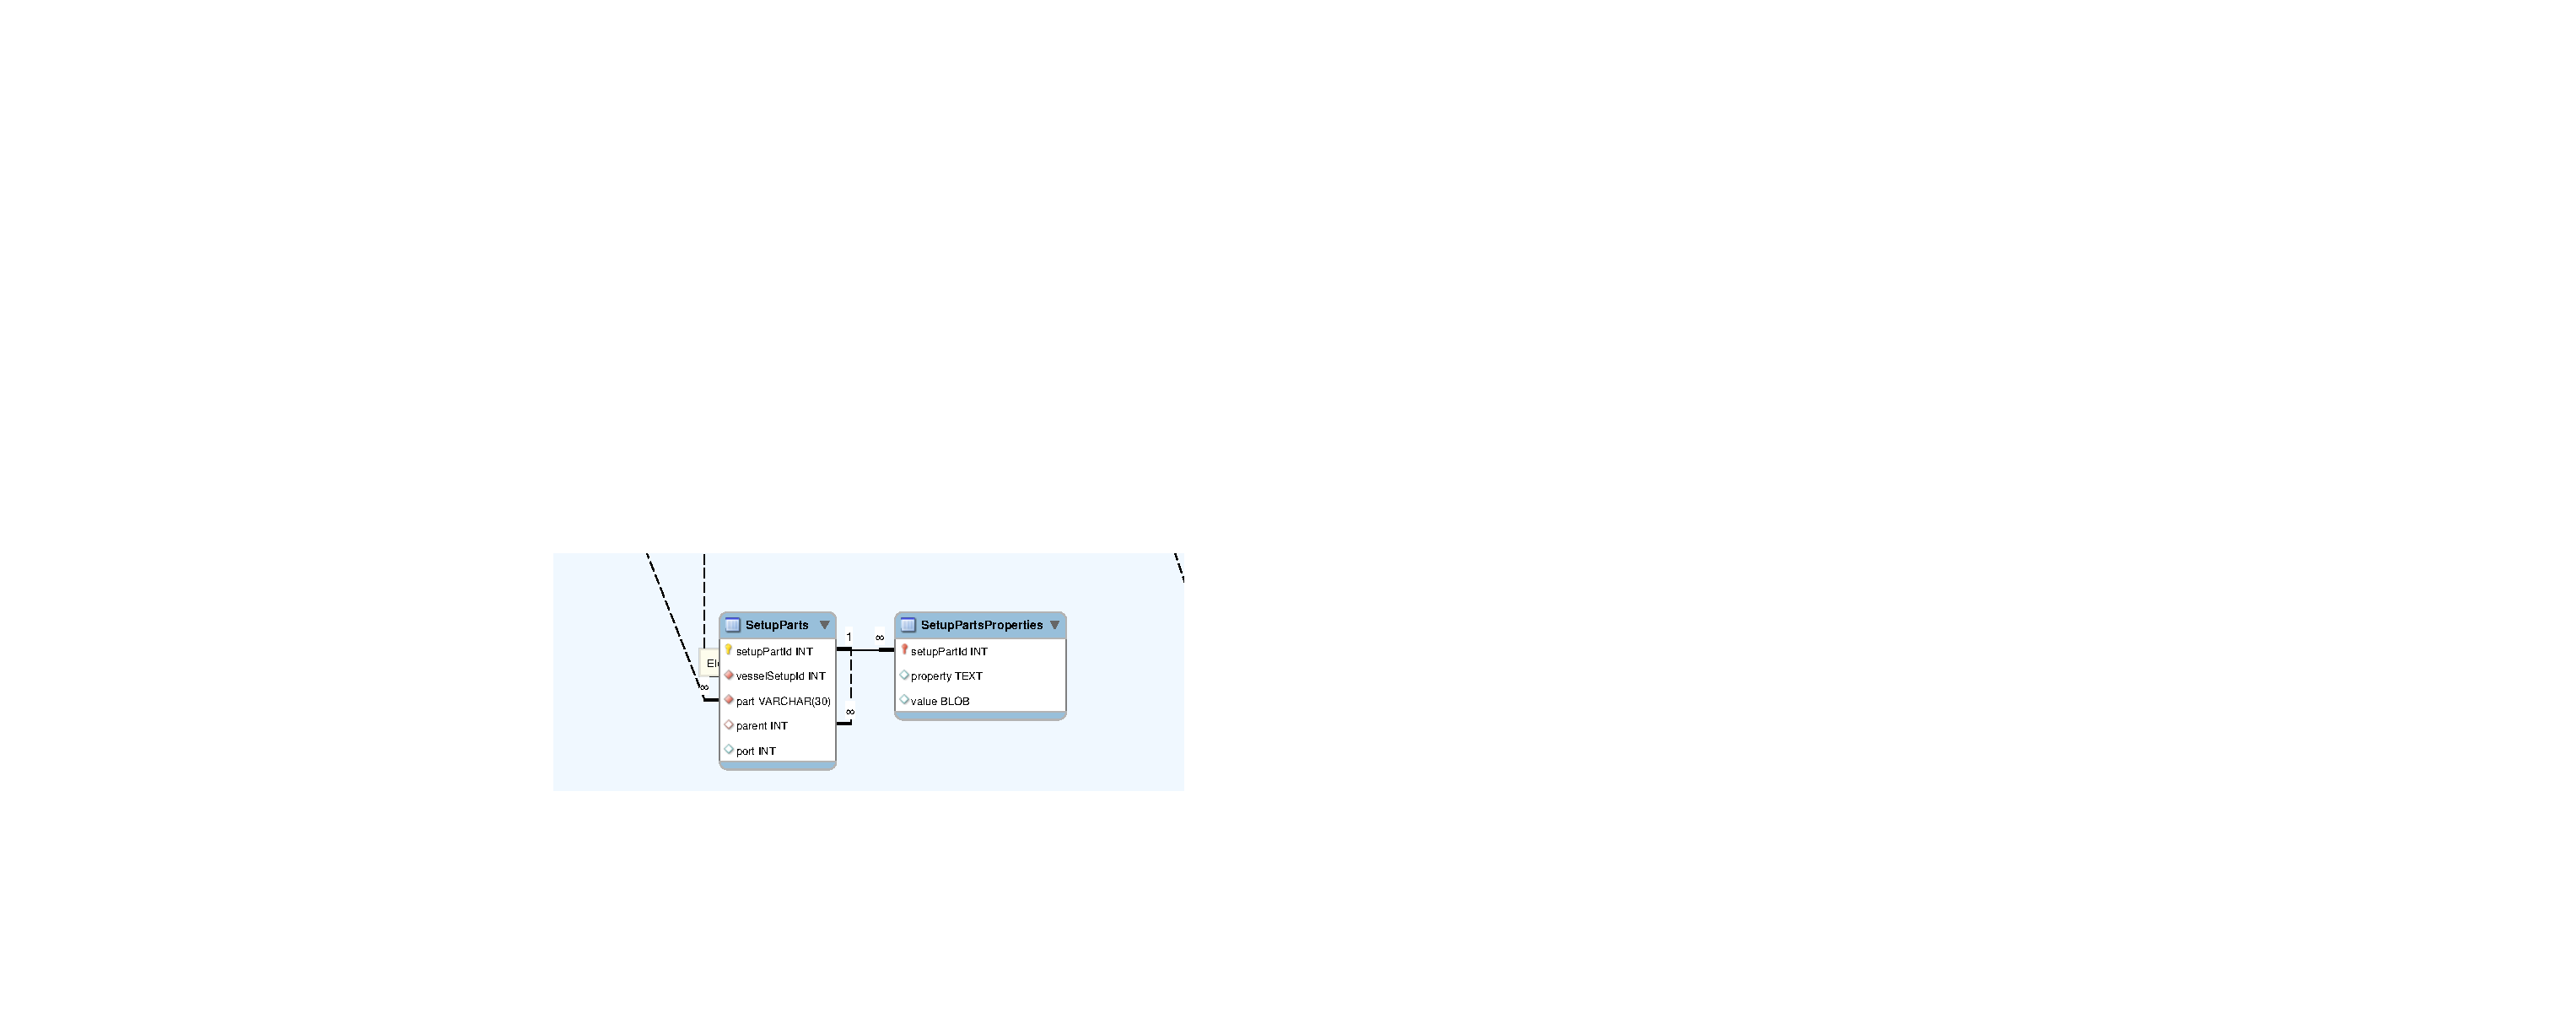
\includegraphics[width=3in]{figures/setup-parts2.pdf}
        %\end{minipage}
    }
    \caption{Two relational approaches to manage data with vastly different attributes}
    \label{setup-parts}
\end{figure}

 Another approach for this is using a properties table, as shown in Figure~\ref{setup-parts-b}, in which a table is used to store the name of the attribute and the value of the attribute for all setup parts. This design is flexible, schema-less, and allow any attribute to be added to any setup parts. One drawback is that, as shown in the figure, we lose the data type information for the values, as now simple stored as a blob type, which means any data.

\subsection{NoSQL and MongoDB}

In recent years, a new category of database systems, called NoSQL (Not Only SQL\footnote{http://en.wikipedia.org/wiki/NoSQL}), have gained popularity in the sphere of web-based applications and services designed to solve the same problem we are facing on our project. NoSQL is a new breed of database systems designed to handle new challenges of managing data of the web. In particular, most NoSQL systems are designed to handle large amount of data, and to support flexible data schema and work with large variety of data\cite{Stonebraker2010}.

Among NoSQL systems, MongoDB\footnote{http://mongodb.org} is a document-based database system that has gained attention in both research and development communities. Despite being categorized as a NoSQL system, MongoDB's data model has similar counterparts in the relational model. The system is composed of multiple databases. For each database, there are multiple collection and each collection holds documents, which are key value pairs. The collections and documents in MongoDB are analogous to tables and records in the relational model.

Of course MongoDB is different from relational database as well. Unlike the relational model, documents in a collection do not need to have the same structure, although it is natural for documents in the same collection to have similar structure. The system supports list structure. In relational model, lists are stored in a separate table referenced by foreign key. The system also supports nested documents; so, in MongoDB it is possible to have a hierarchical structure of documents.

\subsection{The Goal of Case Study}

In this case study, we present our findings during our database migration from MySQL database to MongoDB. We first present the rationale for schema changes, followed by performance evaluation to compare the performance of the two version of the system.


%\section{Relate Works}

\section{MongoDB Data Model}

MongoDB was designed to be distributed database system where data can be distributed across different machines or different instances of the software on a single machine. In this preliminary study, we only consider data on a single machine and single server instance.

A single server instance contains multiple databases. A MongoDB database is similar to a MySQL database, which holds categories of data for a particular project (or application). For example, all data in our MDPX project is current held in a single MySQL database.

A single MongoDB database holds a set of collections. A MongoDB collection is similar to a table in relational databases. A collection holds a set of documents, which are the actual data in the database. A collection hold documents of similar properties and structure, but keep in mind, MongoDB does not enforce data schema; therefore a single collection could hold documents of completely different structures. Also a database could only have one collection that holds all kinds of documents. However, the data can be more efficiently indexed and queried to be divided into collections of similar documents.

A collection holds a set of JavaScript Object Notation (JSON) documents. The name document may convey the idea that data is textual, but it is not the case. A JSON document is a set of key-value pairs. The key is attribute name, and the value is the data of the attribute. Listing~\ref{json} shows an example of JSON document of a publication.

\begin{lstlisting}[float,caption=A simple JSON document, label=json]
{
    'title':'Anonymous Sensory Data Collection',
    'authors':['Chih-Jye Wang', 'Wei-Shinn Ku'],
    'year':2012
    'talk':
    {
        'conference': 'ICDE',
        'city': 'Washington, D.C.'
    }
}
\end{lstlisting}

In Listing~\ref{json}, `title', `authors', `year', and `talk'. The values follow the keys. In addition to character and numeric data types, JSON also support lists, as in the authors field, and documents, as in the talk field in the example.

% MongoDB does not support joins

\section{Schema Migration}
\subsection{Normalization and De-normalization}

Normalization is a term that is almost inseparable with the relational database and highly recommended during relational data modeling. It is the practice of dividing and organizing data into cohesive relations. For example the user and user role in our project are stored in separate tables. This is because user roles can be applied and assigned to multiple users. With normalized data, it is easy to make modification to the user roles table, for example adding a permission, and the change apply to all users with the same role. The point for normalization is to keep a piece data in only one place, so that data update is simple and there is no copies of the same data to be synchronized.

MongoDB, however, advocates the opposite approach. The relational model forces developers to normalize their design because lists and nested data are unnatural in tables. However, MongoDB allows both lists and nested document inside a document; so, if we want, we don't ever have to normalize.

In addition, MongoDB does not support joins as a query operation. This is one of the biggest distinction between MongoDB and relational databases, and biggest difference for document-based data design. To join two documents, the user would have to make multiple queries (at least 2): the first query to retrieve the referencing document, then subsequent queries for referenced document.

There are benefits of de-normalization (not normalizing). Joins are often one the most expensive operation when searching for data\cite{Mishra1992, Aho1979}. When data becomes large, joins have to search a large number of records for join. Keep in mind, MongoDB is design for big data of the web; therefore, it makes sense, in term of query performance, that MongoDB does not support joins. In short, normalization makes update more efficient; whereas de-normalization makes reads more efficient.

\subsection{Proposed Changes}

Despite MongoDB's inability to perform joins, we still have to keep our data consistent and not doing more work than we have to when updating data. We do not want to start de-normalizing our original schema into one big blob of data. Instead we want to keep data normalized where we think change (updates) will be common and we can combine tables where updates are almost never made.

The following changes are proposed.

\begin{enumerate}
\item Combine 3 tables into Part: (PartCategories, Parts, ChamberSides) $\rightarrow$ Part.
\item Combine 4 tables into Setup: (ExperimentSetups, VesselSetups, SetupParts, SetupCameras, SetupProbes) $\rightarrow$ Setup.
\end{enumerate}

Figure~\ref{proposed-schema} shows the document-based schema after the proposed changes. Keep in mind, the figure is a rough schema to show document structures using relational notation; therefore lists and sub-documents structures are not shown. Detailed document structures will be illustrated in the remainder of this section as we go into details of the changes.

\begin{figure}[h]
\begin{center}
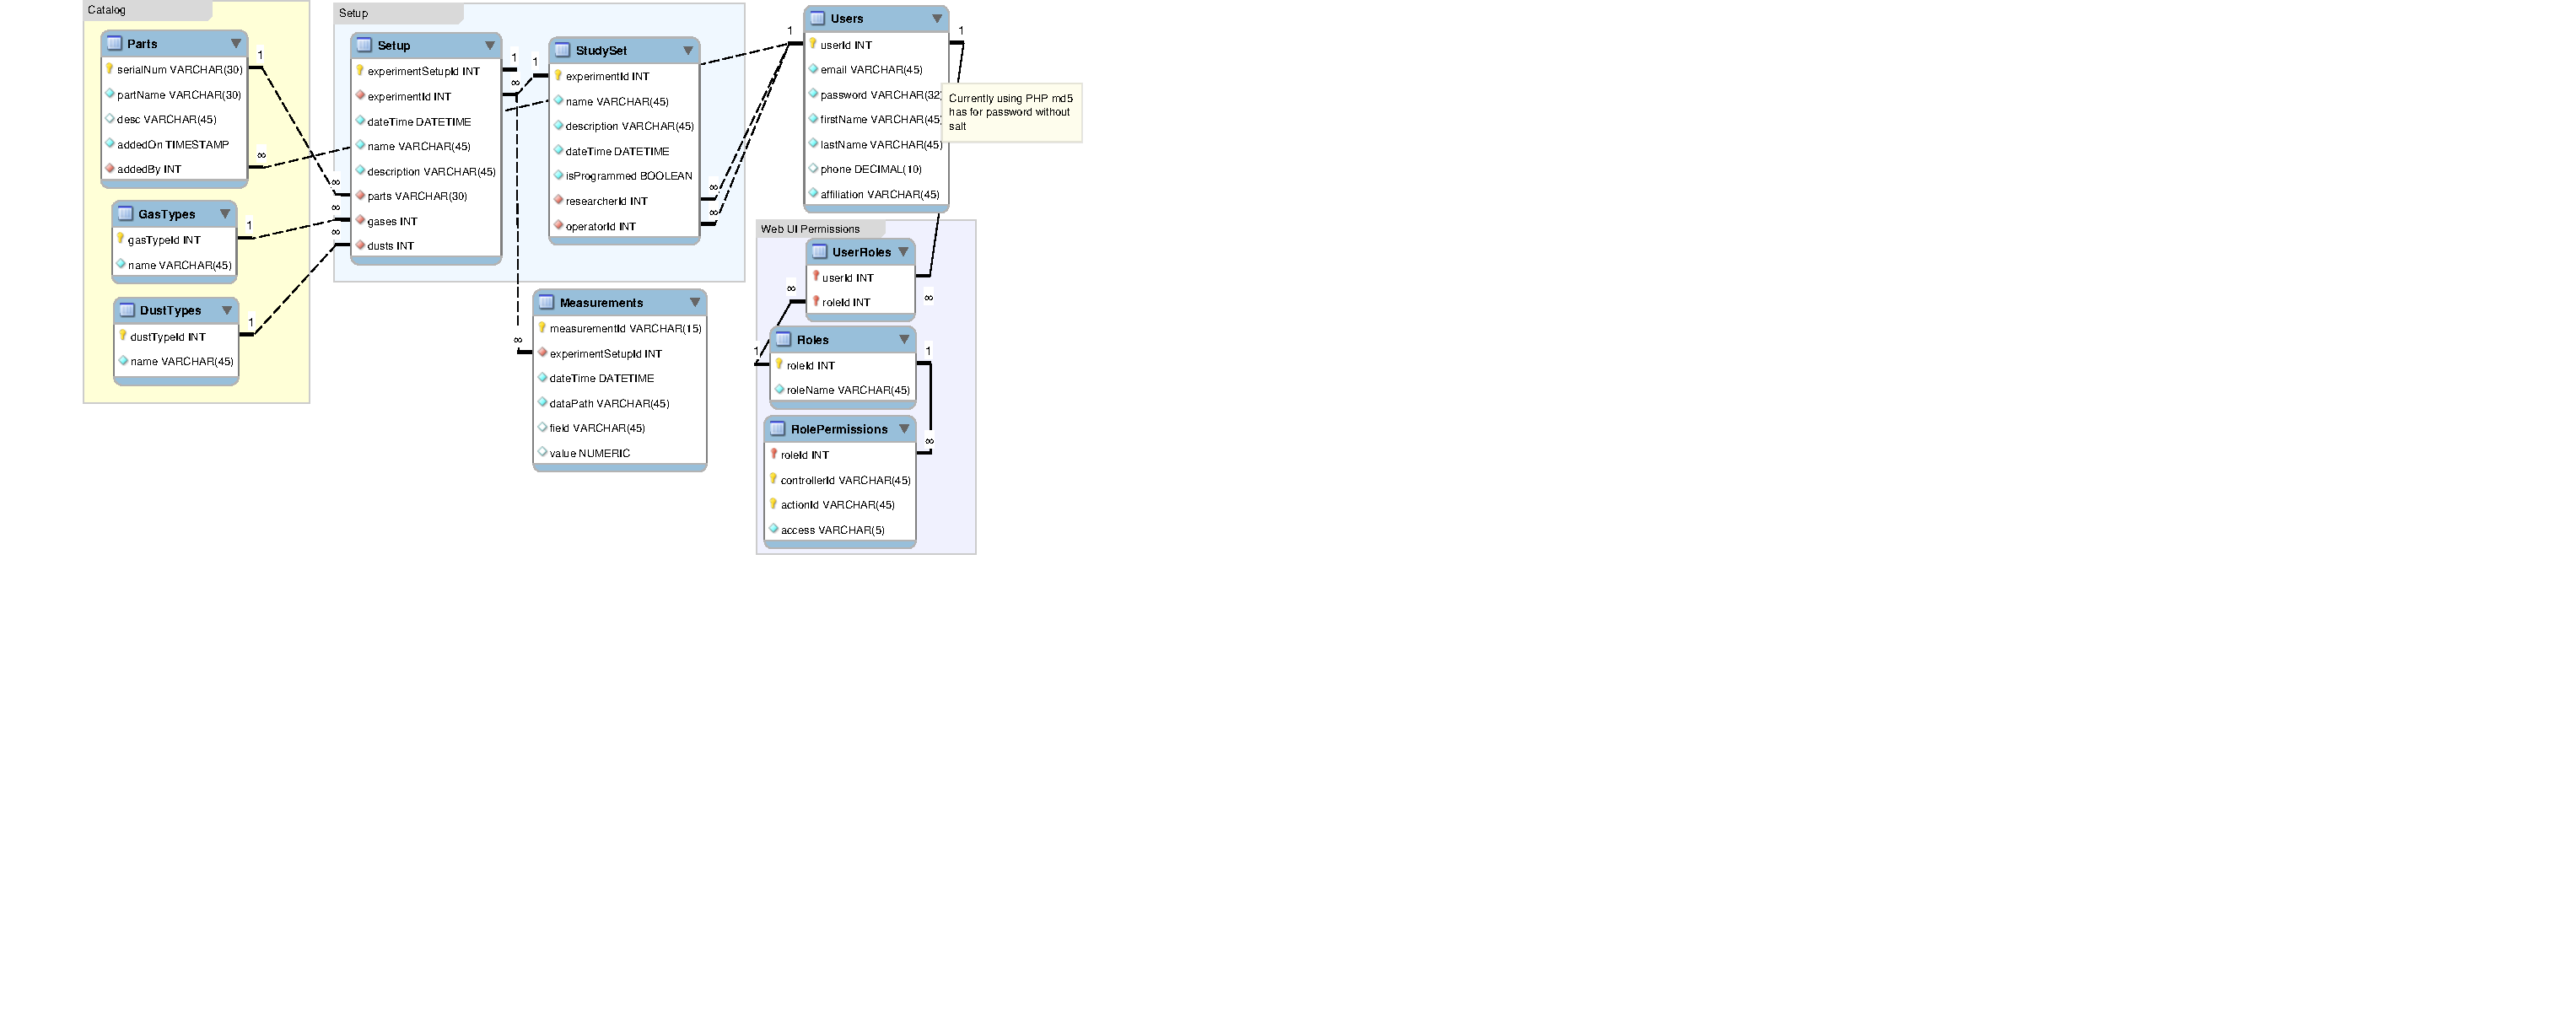
\includegraphics[width=6in]{figures/doc-schema.pdf}
\caption{Proposed document-based schema.\label{proposed-schema}}
\end{center}
\end{figure}

\subsubsection{Part Documents }

In the part catalog section (proposed change 1 in the list), two tables were removed (merged into Part document). The first is the PartCategories table. In the previous schema design, we had a part categories table for two purposes. The first is that we can query based on broader categories. For example, querying all experiments with cameras, without specifying a specific kind of camera. However, this is not typically how a user query about parts. The reason is that, most experiments have several broad categories of parts and user often query based on a specific part (for example, most setup have a chamber, electrodes, cameras, etc). If querying based on broad category is needed, an user can perform regular expression matching on the part serial number. The second use for the table is when adding a new part to the catalog, the system is able provide a list of all the parts that can be added, which are queried from PartCategories table. However, we found this step to be redundant and we can just allow user to enter part name and other part information directly. Also a list of parts can also be populated from the Part collection directly, as the collection become populated.

The second table that has been removed is the ChamberSides table. The purpose of this table was to annotate side information of chamber parts. Due to the fact that a document can contain any number of fields, we decided such annotation can be additional fields in the unified Part table. The consequence of this is that the documents in the new Part collection may have different number of fields depending on the part, but at least the basic fields shown in the proposed schema will be there.

\subsubsection{Setup Documents}

This section is the biggest change in our schema. This was also the most complicated part of our original schema because these tables record how parts are connected in an experiment and the settings (set-points) on the parts. Essentially we decided to merge all part setup tables into one because most of these data do not change once they are inserted into the database. Having all these information stored in a single document eliminates most query joins and could improve query efficiency.

We merged VesselSetups and its sub-tables: SetupParts, CameraSetups, and SetupProbes. This portion of the schema was the original motivation to move to MongoDB. This change makes sense because after the change, we no longer need one table for each part type. Once again this change is possible because documents do not have a set format. For each part, we would have different fields to describe that part. Listing~\ref{setup-document} shows a sample document in this collection. Line 7 of the sample shows an electrode part with an attribute `DC Voltage' and Line 11 show a camera part with complete different attributes `positionR' and `positionZ' describing the part.

\begin{lstlisting}[float,caption=Sample document for the Setup collection, label=setup-document]
{
    '_id'    : ObjectId("5037ee4a1084eb3ffeef7228"),
    'time'   : ISODate("2012-08-24T21:12:09.982Z"),
    'name'   : 'Study 1',
    'desc'   : 'Study 1 description',
    'parts'  : [
        {'partNum' : 'xyz123', 'partName' : 'Upper Electrode', 'DC Voltage' : 10},
        {'partNum' : 'vac111', 'partName  : 'Octagon Chamber',
            'parts' : [
                {'partNum' : 'winblnk', 'partName' : 'Window Blank', 'port' : 1},
                {'partNum' : 'cam1234', 'partName' : 'Camera123'   , 'port' : 1, 'positionR' : 50, 'positionZ' : 60},
                ...
            ], ...
        }
    ],
    'gasses' : [...],
    'dusts'  : []
}
\end{lstlisting}

The second change is that we embedded the parts hierarchy directly in the Setup document. In the previous design the hierarchy was described by VesselSetups and it's child table SetupParts, which is self-referencing that forms the hierarchy. In the new structure, each Setup document contains a `parts' field, which is an array (list) of part documents. Each part sub-document, also contains a list of parts that are connected to that part and so on and this forms the hierarchy. Take Listing~\ref{setup-document} for example: line 8 of the sample document shows a part with partNum = `vac111' that has 2 sub-parts, which have partNum `winblnk' and `cam1234'.
 
Third, we remove the set-point fields from the original ExperimentSetups table. These fields are the following:

\begin{enumerate}
\item dcVaoltageSetpoint
\item dcCurrentSetupPoint
\item rfPowerSetPoint
\item pressureSetpoint
\item magnet1Setpoint
\item magnet2Setpoint
\item magnet3Setpoint
\item magnet4Setpoint
\item magneticFieldSetpoint
\item magneticFieldGradientSetupoint.
\end{enumerate}

We removed this fields because we believe these can be described by the parts hierarchy. We renamed the table Experiments to StudySet, which reflects better the purpose of the collection. We did not touch the user management and access control portion of the schema.

\section{Evaluation}

\subsection{Experiment Design}

In this section we describe our evaluation design. In the previous section, it is clearly seen that our migration from MySQL to MongoDB significantly simplify the database schema. The goal of the evaluation is to compare the running time performance of the two systems.

Experiments are divided into two parts: data insertion, and data query. The goal of the insertion evaluation is to test the write speed of both MySQL and MongoDB. For this part, we insert synthetically generated data sets of parts of size 100, 200, 400, 800, and 1000. The running time are recorded.

For the query evaluation, we want to target three kinds of query operations. The first is a simple query that involves only one collection (table), and no join operation. This would be querying the records of the parts table we inserted earlier.

The second kind of query is query that do involve join operations. There are still a few collections in our schema that contains references to other collections. The simplest one is User and UserRole collection. We use these for our evaluation.

The third kind of query we want to evaluate is aggregations. Aggregations are like getting the sum of certain field. Aggregation in MySQL is very easy and native to the system; on MongoDB however, it is different because of the varying document structure, MongoDB only supports limited aggregation capability but allow the developer to write custom aggregation routines utilizing Hadoop. More study will be needed on this part and we will finalized the aggregation routine we are going to run for this part of evaluation.

\section{Conclusion}

% Related Works
% Schema Migration (?)
%    Pro and Con
%    Rationale
%    Characteristic of MongoDB
%    Consideration
%    Would be MongoDB schema
% Evaluation of Two Databases
%    Insertion
%    Simple no join query
%    Join queries
%    Aggregation (?)
%    Storage efficiency
